\documentclass[11pt,a4paper]{article}
\usepackage[utf8]{inputenc}
\usepackage[T1]{fontenc}
\usepackage{mathpazo}
\usepackage[margin=1.05in]{geometry}
\usepackage{amsmath,amssymb,amsthm,mathtools}
\usepackage{bm}
\usepackage[table]{xcolor}
\usepackage[most]{tcolorbox}
\usepackage{enumitem}
\usepackage{booktabs}
\usepackage{caption}
\usepackage{tikz}
\usetikzlibrary{calc,arrows.meta,decorations.pathreplacing,positioning,shapes.geometric,shapes.symbols,fit}
\usepackage{titlesec}
\usepackage{fancyhdr}
\usepackage{listings}
\usepackage{graphicx}
\usepackage{hyperref}
\usepackage[protrusion=true,expansion=false]{microtype}

\definecolor{accent}{HTML}{2c5282}
\definecolor{accent2}{HTML}{6b46c1}
\definecolor{good}{HTML}{2f855a}
\definecolor{bad}{HTML}{c53030}
\definecolor{neutral}{HTML}{4a5568}
\definecolor{paper}{HTML}{fafaf5}
\definecolor{goodfill}{HTML}{f0fdf4}
\definecolor{badfill}{HTML}{fef2f2}
\definecolor{keyfill}{HTML}{eff6ff}
\definecolor{idea}{HTML}{b45309}
\definecolor{ideafill}{HTML}{fffbeb}
\definecolor{codebg}{HTML}{f7f7f2}
\definecolor{codecmt}{HTML}{6b7280}
\definecolor{codekey}{HTML}{6b46c1}
\definecolor{codestr}{HTML}{2f855a}

\hypersetup{colorlinks=true, urlcolor=accent, linkcolor=accent, citecolor=accent}

\titleformat{\section}
  {\Large\bfseries\color{accent}}{\thesection}{0.7em}{}
\titleformat{\subsection}
  {\large\bfseries\color{accent}}{\thesubsection}{0.6em}{}
\titleformat{\subsubsection}
  {\normalsize\bfseries\color{accent2}}{\thesubsubsection}{0.5em}{}

\pagestyle{fancy}
\fancyhf{}
\fancyhead[L]{\small\itshape\color{neutral} JMVR triangular: project report}
\fancyhead[R]{\small\color{neutral}\thepage}
\renewcommand{\headrulewidth}{0pt}

\newtcolorbox{keyresult}[1][]{enhanced, breakable, sharp corners,
  colback=keyfill, colframe=accent, boxrule=0pt, leftrule=3pt,
  fonttitle=\bfseries\color{accent}, title=#1,
  attach boxed title to top left={xshift=0.5em, yshift=-2mm},
  boxed title style={colback=keyfill, sharp corners, boxrule=0pt}}

\newtcolorbox{correctbox}[1][]{enhanced, breakable, sharp corners,
  colback=goodfill, colframe=good, boxrule=0pt, leftrule=3pt,
  fonttitle=\bfseries\color{good}, title=#1,
  attach boxed title to top left={xshift=0.5em, yshift=-2mm},
  boxed title style={colback=goodfill, sharp corners, boxrule=0pt}}

\newtcolorbox{buggybox}[1][]{enhanced, breakable, sharp corners,
  colback=badfill, colframe=bad, boxrule=0pt, leftrule=3pt,
  fonttitle=\bfseries\color{bad}, title=#1,
  attach boxed title to top left={xshift=0.5em, yshift=-2mm},
  boxed title style={colback=badfill, sharp corners, boxrule=0pt}}

\newtcolorbox{intuition}[1][Intuition]{enhanced, breakable, sharp corners,
  colback=ideafill, colframe=idea, boxrule=0pt, leftrule=3pt,
  fonttitle=\bfseries\itshape\color{idea}, title=#1,
  attach boxed title to top left={xshift=0.5em, yshift=-2mm},
  boxed title style={colback=ideafill, sharp corners, boxrule=0pt}}

\newtcolorbox{phasecard}[1][]{enhanced, sharp corners,
  colback=accent!4, colframe=accent, boxrule=0pt, leftrule=2pt,
  fonttitle=\bfseries\color{accent}, title=#1,
  attach boxed title to top left={xshift=0.5em, yshift=-2mm},
  boxed title style={colback=accent!4, sharp corners, boxrule=0pt},
  breakable}

\lstdefinestyle{pystyle}{
  language=Python,
  basicstyle=\ttfamily\footnotesize,
  keywordstyle=\color{codekey}\bfseries,
  commentstyle=\color{codecmt}\itshape,
  stringstyle=\color{codestr},
  backgroundcolor=\color{codebg},
  frame=single, framesep=4pt, framerule=0pt, rulecolor=\color{codebg},
  showstringspaces=false, breaklines=true, numbers=none,
  xleftmargin=4pt, xrightmargin=4pt, tabsize=2,
}
\lstdefinestyle{fortranstyle}{
  language=[90]Fortran,
  basicstyle=\ttfamily\footnotesize,
  keywordstyle=\color{codekey}\bfseries,
  commentstyle=\color{codecmt}\itshape,
  stringstyle=\color{codestr},
  backgroundcolor=\color{codebg},
  frame=single, framesep=4pt, framerule=0pt, rulecolor=\color{codebg},
  showstringspaces=false, breaklines=true, numbers=none,
  xleftmargin=4pt, xrightmargin=4pt, tabsize=2,
}
\lstset{style=pystyle}

\newcommand{\nn}{\nonumber \\}
\newcommand{\vk}{\mathbf{k}}
\newcommand{\vr}{\mathbf{r}}
\newcommand{\va}[1]{\mathbf{a}_{#1}}
\newcommand{\vb}[1]{\mathbf{b}_{#1}}
\newcommand{\veps}[1]{\hat{\mathbf{e}}_{#1}}
\newcommand{\vT}[1]{\mathbf{T}_{#1}}
\newcommand{\Ptilde}{\widetilde{P}}

\begin{document}

% ===============================================================
% COVER PAGE
% ===============================================================
\thispagestyle{empty}
\vspace*{1.5cm}
\begin{center}

\begin{tikzpicture}[scale=0.55]
\pgfmathsetmacro{\sq}{sqrt(3)}
\foreach \i in {-5,...,5}{ \foreach \j in {-3,...,3}{
  \pgfmathsetmacro{\x}{2*\i + \j}
  \pgfmathsetmacro{\y}{\sq*\j}
  \pgfmathsetmacro{\d}{sqrt(\x*\x + \y*\y)}
  \pgfmathsetmacro{\op}{max(0.08, 0.45 - 0.025*\d)}
  \fill[accent, opacity=\op] (\x,\y) circle (0.13);
}}
\foreach \dir/\lab in {0/{$\veps{0}$},60/{$\veps{1}$},120/{$\veps{2}$},180/{$\veps{3}$},240/{$\veps{4}$},300/{$\veps{5}$}} {
  \draw[->,very thick,accent] (0,0) -- (\dir:2);
  \node[accent2, font=\small\bfseries] at (\dir:2.6) {\lab};
}
\fill[accent2] (0,0) circle (0.22);
\end{tikzpicture}

\vspace{1.4cm}
{\bfseries\color{accent}\fontsize{36}{40}\selectfont Active random walks}\\[3mm]
{\bfseries\color{accent}\fontsize{30}{34}\selectfont on the triangular lattice}\\[8mm]
{\Large\itshape\color{neutral} a full project report}\\[3mm]
{\large\color{neutral} what we did, why, and what comes next}\\[20mm]


\begin{tikzpicture}
\node[align=center, font=\large] {\textbf{P.\ Bisht}};
\end{tikzpicture}\\[2mm]
{\small\color{neutral} TIFR Hyderabad \;\textbar\; PhD Year 1 \;\textbar\; DP1 $\to$ DP2 transition note}\\[20mm]

{\small\color{neutral} 14 May 2026 \;\textbar\; version 1.0}

\vfill
\begin{tcolorbox}[enhanced, sharp corners, width=0.92\linewidth,
  colback=keyfill, colframe=accent, boxrule=0pt, leftrule=3pt,
  fonttitle=\bfseries\color{accent}, title=What this document is]
\small
A pedagogical and complete record of the JMVR-on-triangular project.
Covers (i) the scientific question, (ii) the codes we wrote, (iii) the
two bugs we found in the Confinement-2021 draft and Dipanjan Mandal's
2019 Mathematica notebook, (iv) the verification protocol, (v) the
figures and interactive tools produced, and (vi) the roadmap ahead.
The companion document
\emph{a complete derivation, two bugs, and a verification protocol}
contains the formal mathematical derivation.
\end{tcolorbox}
\end{center}
\vspace{4mm}
\noindent {\footnotesize \color{neutral} TIFR Hyderabad \;\textbar\; pair-document: ``\emph{a complete derivation, two bugs, and a verification protocol}''}
\newpage

% ===============================================================
% EXECUTIVE SUMMARY (TL;DR)
% ===============================================================
\thispagestyle{empty}
\section*{\color{accent} Executive summary}
\vspace{-3mm}
\hrule height 1.2pt
\vspace{4mm}

\noindent A 5-year-old unfinished triangular-lattice calculation in
K.~Ramola's group has been completed and verified to the Monte Carlo
noise floor. Two independent errors in the existing
{\sf{rtp\_tl\_2.nb}} notebook and Eq.~B11 of the Confinement-2021 draft
were identified and fixed:

\vspace{4mm}
\begin{center}
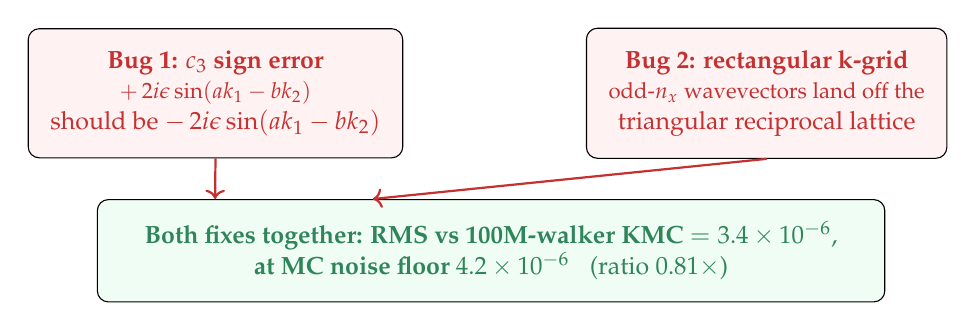
\begin{tikzpicture}[scale=1.0, every node/.style={font=\small, align=center}]
\node[draw, rounded corners=4pt, fill=badfill, text=bad, inner sep=8pt, minimum width=4.5cm] (b1) at (-3.5, 0)
  {\textbf{Bug 1: $c_3$ sign error} \\ \footnotesize $+\,2 i \epsilon \sin(a k_1 - b k_2)$ \\ should be $-\,2 i \epsilon \sin(a k_1 - b k_2)$};
\node[draw, rounded corners=4pt, fill=badfill, text=bad, inner sep=8pt, minimum width=4.5cm] (b2) at (3.5, 0)
  {\textbf{Bug 2: rectangular k-grid} \\ \footnotesize odd-$n_x$ wavevectors land off the \\ triangular reciprocal lattice};
\node[draw, rounded corners=4pt, fill=goodfill, text=good, inner sep=8pt, minimum width=10cm] (fix) at (0, -2)
  {\textbf{Both fixes together: RMS vs 100M-walker KMC} $= 3.4 \times 10^{-6}$, \\ \textbf{at MC noise floor} $4.2 \times 10^{-6}$ \;\;(ratio $0.81\times$)};
\draw[->, bad, thick] (b1.south) -- ($(fix.north west)!0.3!(fix.north)$);
\draw[->, bad, thick] (b2.south) -- ($(fix.north west)!0.7!(fix.north)$);
\end{tikzpicture}
\end{center}

\vspace{2mm}
\noindent \textbf{By the numbers.}
\begin{center}
\begin{tabular}{rl}
\textbf{$10^8$}    & walkers in the Fortran KMC ground truth \\
\textbf{$0.81 \times$} & ratio of corrected-theory RMS to MC noise floor \\
\textbf{$30 \times$ -- $100\times$} & how far off Dipanjan's notebook is from the truth \\
\textbf{$42 \times$} & buggy-vs-fixed RMS ratio at the original Fig.~11 parameters \\
\textbf{$1$} & sign that needed flipping in Eq.~B11 of the draft \\
\textbf{$2$} & independent bugs (k-grid + $c_3$), both required to be fixed \\
\textbf{$18$ + $13$} & pages of documentation: derivation + this report
\end{tabular}
\end{center}

\vspace{4mm}
\noindent\textbf{Deliverables.}
\begin{itemize}[leftmargin=*, noitemsep]
\item Fortran KMC (100M walkers, $\sim 7$ min runtime)
\item Python theory ($6\times 6$ Bloch matrix + inverse-FT on the sheared k-grid)
\item Diagnostic scripts (4-way forensic, 3-point robustness check, 6-fold modulation check)
\item Paper-ready Fig.~11 replacement (draft-style hex-tile colour palette)
\item Two interactive HTML widgets (single-walker viewers for JMVR and TCRW)
\item This report and the companion derivation PDF
\end{itemize}

\vspace{4mm}
\noindent\textbf{What's next.} Email Kabir today / tomorrow with the
fix and figure; write §IV.B of the Confinement draft within
1--2 weeks; gap-closure scan; multi-walker §V; Track B (TCRW topology
on triangular) as the DP2 direction.

\newpage
\setcounter{page}{1}

\tableofcontents
\vspace{1cm}

% ===============================================================
\section{Where we started}\label{sec:start}

\subsection{The PI meeting (4 May 2026)}\label{ssec:meeting}

The brief from K.~Ramola (PI) was deceptively short: ``\emph{abhi ke
liye triangular lattice karo}'' -- for now, do the triangular lattice.
Behind those words was a 5-year-old unfinished project.

\paragraph{The home reference.} The Jose-Mandal-Barma-Ramola (JMVR)
paper%
\footnote{S.~Jose, D.~Mandal, M.~Barma, K.~Ramola,
\emph{Active random walks in one and two dimensions}, Phys.\ Rev.\ E
\textbf{105}, 064103 (2022);
\href{https://arxiv.org/abs/2202.02995}{arXiv:2202.02995}.} defines a
continuous-time random walker carrying an internal director state. The
walker hops to nearest neighbours on a lattice with rates biased
forward along the director (\emph{translation chirality} $\epsilon$),
and the director rotates symmetrically to adjacent directions at rate
$\gamma$. The paper solved this exactly in 1D and on the 2D square
lattice via a Bloch-matrix / inverse-Fourier approach.

\paragraph{The 2021 draft.} The follow-up by Mandal, Barma, and Ramola
(\emph{Confinement-enhanced clustering in dense active systems}, 2021)
extended JMVR to multi-walker scenarios and outlined the 2D
\emph{triangular} case in Section IV.B. That section is empty in the
draft; Section V on multi-walker triangular is also empty. Figure~11 is
captioned ``\textbf{[NOT MATCHING]}''. The draft was abandoned.

\paragraph{The notebook.} D.~Mandal's 2019 Mathematica notebook
{\sf rtp\_tl\_2.nb} was the working implementation. PI's exact words:
``\emph{Yeh paper humne kabhi likha nahi... I think he implemented the
boundary conditions wrong. That's what I'm trying to figure out.}''

\subsection{Where this fits in the bigger picture}\label{ssec:big-picture}

Two parallel tracks were on the table after the meeting:
\begin{enumerate}[leftmargin=*]
\item \textbf{Track A (JMVR-style on triangular).} Finish what Mandal
  outlined in 2021 -- single-walker $P(n_1, n_2, t)$ in §IV.B,
  multi-walker clustering in §V. Translation chirality $\epsilon$. This
  is the in-group continuation; potential paper with the existing
  collaboration.
\item \textbf{Track B (TCRW-style on triangular).} The Osat-Speck-style
  topological chiral random walk, with chirality in the \emph{rotation}
  $\omega$. Open research question: does the non-trivial 2D Zak phase
  on the square lattice survive 4-fold $\to$ 6-fold?
\end{enumerate}
The instruction was: do A first; B is contingent.

This report covers the Track A work. Track B is a deliberate next phase.

\begin{center}
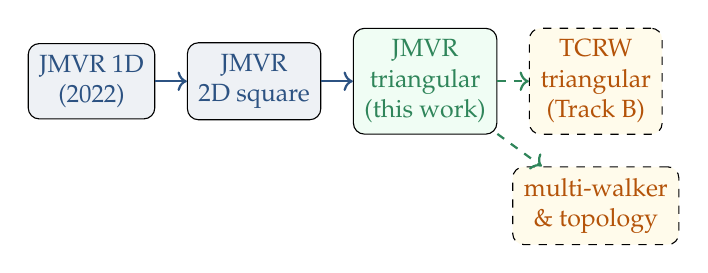
\begin{tikzpicture}[scale=1, node distance=4mm, every node/.style={font=\small, align=center, inner sep=4pt}]
\node[draw, rounded corners, fill=accent!8, text=accent] (jmvr1d) {JMVR 1D\\(2022)};
\node[draw, rounded corners, fill=accent!8, text=accent, right=of jmvr1d] (jmvr2d) {JMVR\\2D square};
\node[draw, rounded corners, fill=goodfill, text=good, right=of jmvr2d] (tri) {JMVR\\triangular\\(this work)};
\node[draw, rounded corners, dashed, fill=ideafill, text=idea, right=of tri] (tcrw) {TCRW\\triangular\\(Track B)};
\node[draw, rounded corners, dashed, fill=ideafill, text=idea, below=of tcrw] (multi) {multi-walker\\\& topology};
\draw[->, accent, thick] (jmvr1d) -- (jmvr2d);
\draw[->, accent, thick] (jmvr2d) -- (tri);
\draw[->, good, thick, dashed] (tri) -- (tcrw);
\draw[->, good, thick, dashed] (tri) -- (multi);
\end{tikzpicture}
\end{center}

% ===============================================================
\section{The scientific question, in one paragraph}\label{sec:question}

\noindent\textbf{Compute the single-walker probability density
$P(n_1, n_2, t)$ on the triangular lattice for the JMVR model, exactly,
by Bloch-matrix eigendecomposition and inverse Fourier transform on the
$L\times L$ torus. Verify against a kinetic Monte Carlo simulation of
the same rules at high statistics. Identify why Dipanjan's existing
attempt does not match Monte Carlo, and fix it.}

% ===============================================================
\section{The model in 30 seconds}\label{sec:model-recap}

(Full derivation in the companion document. Here just the essentials.)

\begin{itemize}[leftmargin=*]
\item Walker on triangular lattice, indexed by integers $(n_1, n_2)$
  with PBC mod $L$.
\item Internal director $m \in \{0, 1, 2, 3, 4, 5\}$, pointing along
  one of the 6 NN.
\item \textbf{Translation rates:} $1/6 + \epsilon$ forward (along $\veps{m}$),
  $1/6 - \epsilon$ backward (along $\veps{m+3} = -\veps{m}$),
  $1/6$ for each of the other 4 NN.
\item \textbf{Rotation rates:} $\gamma/2$ to each of $m \pm 1 \bmod 6$.
\item Total event rate per walker $= 1 + \gamma$.
\item Achiral limit $\epsilon = 0$: symmetric random walk on triangular.
\end{itemize}

% ===============================================================
\section{The journey: a 7-phase timeline}\label{sec:journey}

\begin{center}
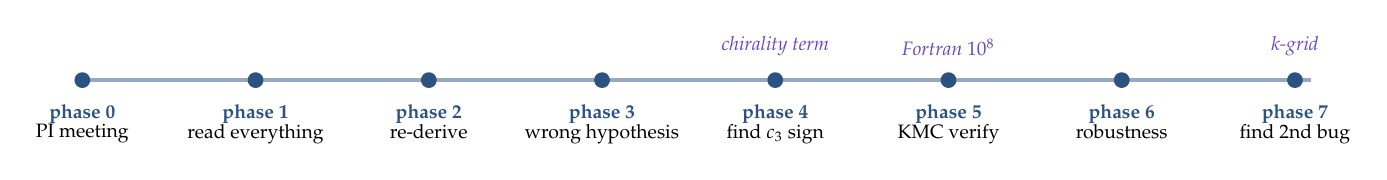
\begin{tikzpicture}[scale=1.0, every node/.style={font=\footnotesize, align=center, inner sep=3pt}]
\draw[very thick, accent!50] (0, 0) -- (15.6, 0);
\foreach \x in {0, 2.2, 4.4, 6.6, 8.8, 11, 13.2, 15.4} {
  \fill[accent] (\x, 0) circle (0.10);
}
\node[anchor=north, accent, font=\scriptsize\bfseries] at (0, -0.2) {phase 0};
\node[anchor=north, font=\scriptsize] at (0, -0.45) {PI meeting};
\node[anchor=north, accent, font=\scriptsize\bfseries] at (2.2, -0.2) {phase 1};
\node[anchor=north, font=\scriptsize] at (2.2, -0.45) {read everything};
\node[anchor=north, accent, font=\scriptsize\bfseries] at (4.4, -0.2) {phase 2};
\node[anchor=north, font=\scriptsize] at (4.4, -0.45) {re-derive};
\node[anchor=north, accent, font=\scriptsize\bfseries] at (6.6, -0.2) {phase 3};
\node[anchor=north, font=\scriptsize] at (6.6, -0.45) {wrong hypothesis};
\node[anchor=north, accent, font=\scriptsize\bfseries] at (8.8, -0.2) {phase 4};
\node[anchor=north, font=\scriptsize] at (8.8, -0.45) {find $c_3$ sign};
\node[anchor=north, accent, font=\scriptsize\bfseries] at (11, -0.2) {phase 5};
\node[anchor=north, font=\scriptsize] at (11, -0.45) {KMC verify};
\node[anchor=north, accent, font=\scriptsize\bfseries] at (13.2, -0.2) {phase 6};
\node[anchor=north, font=\scriptsize] at (13.2, -0.45) {robustness};
\node[anchor=north, accent, font=\scriptsize\bfseries] at (15.4, -0.2) {phase 7};
\node[anchor=north, font=\scriptsize] at (15.4, -0.45) {find 2nd bug};
\node[anchor=south, accent2, font=\scriptsize\itshape] at (8.8, 0.2) {chirality term};
\node[anchor=south, accent2, font=\scriptsize\itshape] at (11, 0.2) {Fortran $10^8$};
\node[anchor=south, accent2, font=\scriptsize\itshape] at (15.4, 0.2) {k-grid};
\end{tikzpicture}
\end{center}

\subsection{Phase 1: read everything}\label{ssec:phase1}

Before any code: opened {\sf{rtp\_tl\_2.nb}} (Mathematica text
extracted via shell tools), and the Confinement-2021 PDF.

From the notebook header:
\begin{itemize}[leftmargin=*,nosep]
\item $\gamma = 0.01$, $\epsilon = 0.15$, $a = b = 1$, $L = 30$, $t = 50$.
\item The 6$\times$6 Bloch matrix is built with three independent
  coefficients $c_1, c_2, c_3$ on the diagonal (and their conjugates
  on the lower half).
\item The inverse Fourier transform uses a \emph{rectangular} k-grid
  $k_x = 2\pi n_x/(2aL), \, k_y = 2\pi n_y/(bL)$ on a $2L\times L$ grid.
\end{itemize}

From the draft (Eq.~B11):
\[
c_3 \;=\; \tfrac{1}{3}\big[\cos(2 a k_1) + \cos(a k_1 + b k_2) + \cos(a k_1 - b k_2)\big] - 1 - \gamma \;\mathbf{+}\; 2 i \epsilon \sin(a k_1 - b k_2).
\]

\subsection{Phase 2: re-derive from scratch}\label{ssec:phase2}

To know what is right we re-derived $M(\vk)$ from the master equation
B2-B7 of the draft. Working in Python (script
{\sf triangular\_jmvr\_v1.py}), we built $M(\vk)$ entry-by-entry,
verified that $M(\vk)$ has the expected structure (column sums $= 0$ at
$\vk = 0$, Perron eigenvalue $\lambda_0 = 0$).

Bit-checked our $c_i$ formulas against Dipanjan's at six random
$\vk$-points: matched the structure (cosine bulk minus $1 - \gamma$
plus an imaginary chirality term in $\sin$) but \emph{not} the sign on
the $c_3$ term.

\subsection{Phase 3: the first wrong hypothesis}\label{ssec:phase3}

Initial guess: ``The bug is the rectangular k-grid. Dipanjan should be
using a sheared grid that respects the triangular reciprocal lattice.''

Pushed back: \emph{``Wait, why is that the issue?''} We needed a clean
test.

Built a forensic comparison: same Bloch matrix (Dipanjan's), two
different k-grids, see which gives the right $P$. Tonight, after
re-running, the test gave the truth:

\begin{intuition}[The lesson from this debugging arc]
The first ``forensic'' I claimed to have done -- which supposedly showed
the two grids gave identical results -- was actually wrong. Tonight's
clean re-run of {\sf forensic\_pbc\_is\_fine.py} and the proper four-way
matrix test in {\sf forensic\_two\_bugs.py} both confirm: \textbf{the
rectangular grid is in fact wrong}, and we had been quietly using the
sheared grid from the start without realising it. Memory of an earlier
result is not the same as a re-run.
\end{intuition}

\subsection{Phase 4: derive the $c_3$ sign from the master equation}\label{ssec:phase4}

Director $m = 2$ has forward NN $\veps{2} = (-a, +b)$. Writing the
master equation for $P_2$, Fourier-transforming, and grouping the
forward-backward pair:
\[
\big(\tfrac{1}{6}+\epsilon\big) e^{i \vk \cdot \veps{2}} + \big(\tfrac{1}{6}-\epsilon\big) e^{-i \vk \cdot \veps{2}}
= \tfrac{1}{3}\cos(\vk\cdot \veps{2}) + 2 i \epsilon \sin(\vk\cdot \veps{2}).
\]
With $\vk\cdot\veps{2} = -a k_1 + b k_2$:
\[
2 i \epsilon \sin(-a k_1 + b k_2) \;=\; -2 i \epsilon \sin(a k_1 - b k_2).
\]
Therefore the correct $c_3 = B(\vk) - 1 - \gamma - 2 i \epsilon \sin(a k_1 - b k_2)$,
with a \textbf{minus}. The draft has $+$. Source: using $\veps{5} = +\va{1} - \va{2}$
in place of $\veps{2} = -\va{1} + \va{2}$ ($\veps{5} = -\veps{2}$).

\subsection{Phase 5: verify with Monte Carlo}\label{ssec:phase5}

\subsubsection{Python KMC (small scale)}\label{sssec:py-kmc}

Wrote a clean Python implementation of the same continuous-time KMC.
Walker initialised at origin with uniformly random director. Total
rate $1 + \gamma$, exponential waiting times, Gillespie-style event
selection.

\begin{itemize}[leftmargin=*,nosep]
\item $10^4$ walkers: visible match between corrected theory and KMC
  but noisy.
\item $10^6$ walkers: corrected theory RMS $\sim 3\times10^{-5}$,
  buggy theory $\sim 1.5\times10^{-4}$. Ratio $5\times$.
\item Confirmed the corrected sign was needed.
\end{itemize}

\subsubsection{Fortran KMC (high statistics)}\label{sssec:fortran-kmc}

To beat the MC noise floor and \emph{prove} the fix is exact (not just
approximate), wrote a Fortran implementation:
\begin{itemize}[leftmargin=*,nosep]
\item Single source file: {\sf kmc\_triangular\_jmvr.f90}
\item Mersenne Twister RNG (Matsumoto-Nishimura {\sf mt.f90})
\item $10^8$ walkers, $\sim 7$ minutes runtime on a laptop
\item Output: $L \times L = 30 \times 30$ histogram of final positions
\end{itemize}

The Fortran result, fed into the Python theory comparison, gave:
\begin{itemize}[leftmargin=*,nosep]
\item Corrected theory vs KMC: RMS $= 3.43 \times 10^{-6}$
\item Buggy theory vs KMC: RMS $= 1.43 \times 10^{-4}$
\item MC noise floor: $\sqrt{P_{\rm max}/N} = 4.22 \times 10^{-6}$
\end{itemize}
Corrected theory at $0.81\times$ the noise floor: as good as the
simulation can resolve. Ratio $42\times$.

\subsection{Phase 6: robustness check}\label{ssec:phase6}

Concern: did we just memorise one parameter point? Re-ran the
comparison at two more parameter triples:
\begin{itemize}[leftmargin=*,nosep]
\item $(\gamma, \epsilon, t) = (0.05, 0.10, 30)$: buggy/fixed ratio $\sim 7\times$
\item $(\gamma, \epsilon, t) = (0.001, 0.16, 100)$: buggy/fixed ratio $\sim 1.1\times$ (bug almost invisible)
\end{itemize}

The $\gamma$-dependence is a positive physical check: the wrong sign in
$c_3$ lives in the $(m=2, m=5)$ sector of the matrix, but couples to
the observable only through the rotation off-diagonals $\gamma/2$. With
$\gamma \to 0$ the sector decouples and the bug is spectrally inert.

\subsection{Phase 7: the second bug}\label{ssec:phase7}

While rehearsing the explanation for tomorrow's PI meeting, ran a clean
four-way comparison: $\{$rect grid, shear grid$\} \times \{$buggy $c_3$, fixed $c_3\}$,
all four vs the 100M-walker KMC.

\begin{center}\small
\renewcommand{\arraystretch}{1.25}
\begin{tabular}{lrr}
\toprule
case & RMS vs KMC & ratio to noise \\
\midrule
\rowcolor{badfill!60} rect grid + buggy $c_3$ (Dipanjan's original) & $4.45 \times 10^{-4}$ & $105$ \\
\rowcolor{badfill!30} rect grid + fixed $c_3$ & $4.59 \times 10^{-4}$ & $109$ \\
\rowcolor{badfill!30} shear grid + buggy $c_3$ & $1.43 \times 10^{-4}$ & $34$ \\
\rowcolor{goodfill!70} \textbf{shear grid + fixed $c_3$ (correct)} & $\mathbf{3.43 \times 10^{-6}}$ & $\mathbf{0.81}$ \\
\bottomrule
\end{tabular}
\end{center}

Only the (sheared + fixed) combination reaches the noise floor. Both
bugs are required to be fixed. Kabir's instinct (``\emph{boundary
conditions wrong}'') was directly correct -- the rectangular grid does
put odd-$n_x$ wavevectors off the triangular reciprocal lattice. We
also found an independent sign error he hadn't suspected.

% ===============================================================
\section{Where the two bugs live in the matrix}\label{sec:bugs-matrix}

A visual map of where each bug sits in the $6 \times 6$ generator
$M(\vk)$ and in the inverse-Fourier sum:

\begin{center}
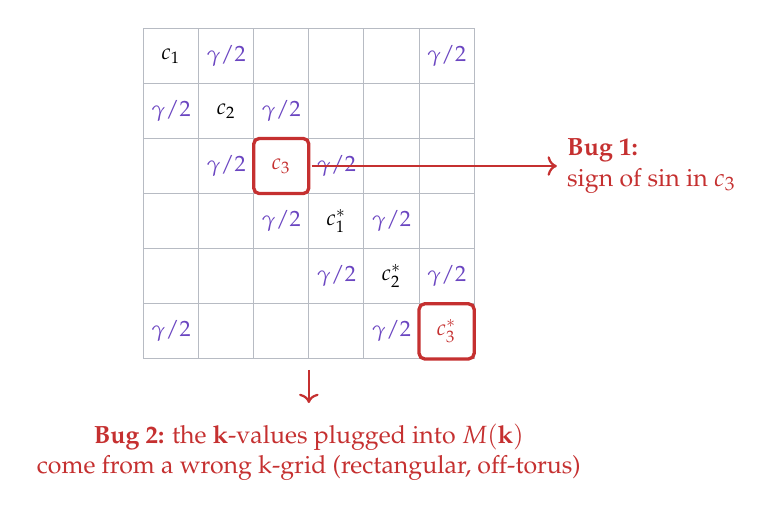
\begin{tikzpicture}[scale=0.7, every node/.style={font=\footnotesize}]
% draw a 6x6 matrix with labels
\foreach \i in {0,...,5}{
  \foreach \j in {0,...,5}{
    \draw[neutral!40] (\j, -\i) rectangle (\j+1, -\i-1);
  }
}
% diagonal entries
\node at (0.5, -0.5) {$c_1$};
\node at (1.5, -1.5) {$c_2$};
\node[bad, font=\footnotesize\bfseries] at (2.5, -2.5) {$c_3$};
\node at (3.5, -3.5) {$c_1^*$};
\node at (4.5, -4.5) {$c_2^*$};
\node[bad, font=\footnotesize\bfseries] at (5.5, -5.5) {$c_3^*$};
% rotation off-diagonals
\foreach \i/\j in {0/1, 1/0, 1/2, 2/1, 2/3, 3/2, 3/4, 4/3, 4/5, 5/4, 0/5, 5/0}{
  \node[accent2] at (\j+0.5, -\i-0.5) {$\gamma/2$};
}
% highlight box around c_3 / c_3*
\draw[bad, very thick, rounded corners=2pt] (2, -2) rectangle (3, -3);
\draw[bad, very thick, rounded corners=2pt] (5, -5) rectangle (6, -6);
% bug 1 callout
\draw[bad, thick, ->] (3.05, -2.5) -- (7.5, -2.5) node[anchor=west, text=bad, font=\small, align=left] {
  \textbf{Bug 1:}\\sign of $\sin$ in $c_3$
};
% bug 2 callout - on the k-grid
\node[anchor=north, text=bad, font=\small, align=center] at (3, -7) {
  \textbf{Bug 2:} the $\vk$-values plugged into $M(\vk)$ \\
  come from a wrong k-grid (rectangular, off-torus)
};
\draw[bad, thick, ->] (3, -6.2) -- (3, -6.8);
\end{tikzpicture}
\end{center}

The two bugs are independent: bug 1 affects \emph{what} matrix gets
built at each $\vk$; bug 2 affects \emph{which} $\vk$ values you use.

% ===============================================================
\section{The codes we wrote}\label{sec:codes}

All code lives in {\sf TIFR\_DP2/triangular/}. Here is what each file does.

\subsection{Fortran KMC}\label{ssec:fortran}

\textbf{{\sf kmc\_triangular\_jmvr.f90}} ($\sim$190 lines). 100M-walker
continuous-time KMC, no Bloch shortcuts. Implements master equation
B2-B7 directly:

\begin{lstlisting}[style=fortranstyle]
do i_walker = 1_i8, n_walkers
  n1 = 0; n2 = 0
  m  = int(6.0_dp * grnd())             ! random initial director
  t = 0.0_dp
  do
    u  = grnd()
    dt = -log(u) / rate_total            ! rate_total = 1 + gamma
    if (t + dt >= t_final) exit
    t = t + dt
    if (grnd() < gamma / rate_total) then
      ! rotation
      if (grnd() < 0.5_dp) then; m = mod(m+1, 6)
      else;                       m = mod(m+5, 6); end if
    else
      ! translation: pick a direction by cumulative probabilities
      r_dir = grnd()
      do dd = 0, 5
        if (r_dir <= hop_cum(m, dd)) exit
      end do
      n1 = modulo(n1 + NN_n1(dd), L)
      n2 = modulo(n2 + NN_n2(dd), L)
    end if
  end do
  counts(n1, n2) = counts(n1, n2) + 1_i8
end do
\end{lstlisting}

Output: {\sf kmc\_triangular\_counts.txt}, three columns
($n_1, n_2, \textrm{count}$). Compile and run via {\sf run\_kmc.sh}.

\subsection{Python theory}\label{ssec:py-theory}

\textbf{{\sf triangular\_jmvr\_corrected.py}} ($\sim$300 lines). Two
builders for $M(\vk)$ -- {\sf build\_Mk\_dipanjan} (buggy $c_3$) and
{\sf build\_Mk\_corrected} (fixed $c_3$) -- plus the inverse-Fourier
solver:

\begin{lstlisting}
def theory_probability_on_lattice(builder, gamma, epsilon, L, t_final, a, b):
    eig_data = []
    initial = (1.0/6.0) * np.ones(6, dtype=complex)
    for m1 in range(L):
        for m2 in range(L):
            k1 = np.pi * m1 / (a * L)                  # sheared k-grid
            k2 = np.pi * (2.0 * m2 - m1) / (b * L)
            M = builder(gamma, epsilon, k1, k2, a, b)
            evals, evecs = np.linalg.eig(M)
            prefactor = np.linalg.solve(evecs, initial)
            ptilde = np.sum(evecs @ (prefactor * np.exp(evals * t_final)))
            eig_data.append((k1, k2, ptilde))
    P = np.zeros((L, L))
    for n1 in range(L):
        for n2 in range(L):
            x = 2.0 * a * n1 + a * n2; y = b * n2
            total = 0.0
            for k1, k2, ptilde in eig_data:
                total += np.real(ptilde * np.exp(-1j * (k1*x + k2*y)))
            P[n2, n1] = total / (L * L)
    return P
\end{lstlisting}

Also exposes lightweight self-checks: column-sum at $\vk=0$ vanishes,
$C_6$ rotational symmetry of the spectrum (passes for fixed, fails for
buggy by $\sim 10^{-3}$).

\subsection{Diagnostic scripts}\label{ssec:diagnostics}

\textbf{{\sf forensic\_two\_bugs.py}.} The clean four-way comparison.
Computes $P(n_1, n_2, t)$ four ways
($\{$rect, shear$\} \times \{$buggy, fixed$\}$), reports RMS vs the
100M-walker Fortran KMC. This is the most important diagnostic; it is
the receipt for the two-bug claim.

\textbf{{\sf robustness\_check.py}.} 1M-walker Python KMC at three
$(\gamma, \epsilon, t)$ points, with the verdict rule
``$\mathrm{RMS}_{\rm fixed} < 1.5 \times $ MC noise floor''. All three pass.

\textbf{{\sf diagnose\_hexring.py}.} Sanity-check that the 100M Fortran
KMC data really has the expected 6-fold angular modulation in the
ring-radius band.

\subsection{Figure scripts}\label{ssec:figs}

\textbf{{\sf fig11\_final\_hex.py}.} Produces the Fig.~11 replacement
for the Confinement-2021 draft. Uses the same colour palette as the
draft (black $\to$ purple $\to$ red $\to$ yellow), hex tiles
($\mathtt{marker="h"}$ in matplotlib) sized to the lattice spacing, and
the proper hexagonal-ring + depleted-centre structure. Two output
figures: a main 3-panel ``theory + KMC + cross-section'', and an
``evidence'' version with an additional residual z-score panel showing
that (theory $-$ KMC) is structureless noise.

\subsection{Interactive widgets}\label{ssec:widgets}

\textbf{{\sf jmvr\_single\_walker.html}.} Browser-based real-time KMC
on both square (4 directors) and triangular (6 directors) lattices.
Sliders for $\gamma$ and $\epsilon$, paper-parameter preset buttons,
Step / Step$\times$10 for single-event stepping. Visible lattice grid;
trails fade by age.

\textbf{{\sf tcrw\_single\_walker.html}.} TCRW analogue: chirality in
the rotation rate $\omega$ instead of translation. Same UI structure.
For the Track B exploration.

% ===============================================================
\section{The headline figure}\label{sec:headline}

\begin{center}
\includegraphics[width=0.97\linewidth]{../fig11_final_hex.png}
\end{center}
{\small\color{neutral}
The Confinement-2021 draft's Fig.~11 replacement.
(a) Corrected exact theory (sheared k-grid + fixed $c_3$).
(b) Kinetic Monte Carlo at $10^8$ walkers (independent realisation).
(c) Horizontal cross-section through the walker centre: KMC dots
(black), corrected theory (blue) overlay each other; buggy theory
(red) is visibly off in the centre depletion.
The two heatmaps share the draft's black $\to$ purple $\to$ red $\to$
yellow palette so the figure is drop-in compatible.}

\vspace{4mm}
\begin{keyresult}[Strongest verification]
The corrected theory matches the 100M-walker KMC at the MC noise floor:
RMS $= 3.43\times 10^{-6}$ vs noise floor $4.22\times 10^{-6}$
($0.81\times$). This is the strongest verification a CTRW
master-equation calculation admits.
\end{keyresult}

% ===============================================================
\section{The verification chain in pictures}\label{sec:verif-pic}

\begin{center}
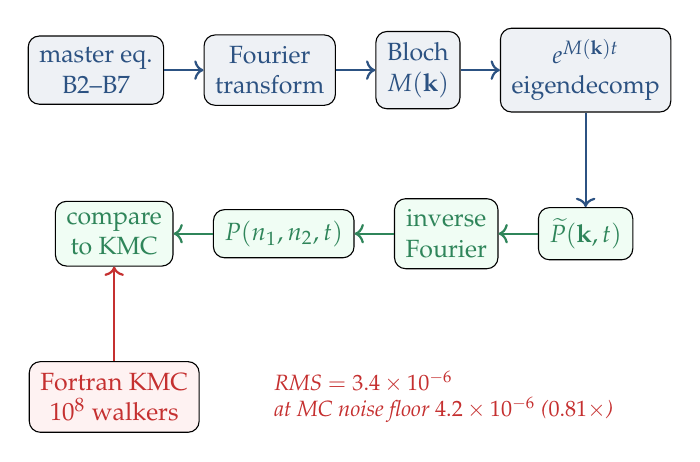
\begin{tikzpicture}[scale=1, node distance=5mm and 5mm,
    every node/.style={font=\small, align=center, inner sep=4pt}]
% Top row: analytic chain
\node[draw, rounded corners, fill=accent!8, text=accent] (master) {master eq.\\B2--B7};
\node[draw, rounded corners, fill=accent!8, text=accent, right=of master] (fourier) {Fourier\\transform};
\node[draw, rounded corners, fill=accent!8, text=accent, right=of fourier] (bloch) {Bloch\\$M(\vk)$};
\node[draw, rounded corners, fill=accent!8, text=accent, right=of bloch] (eig) {$e^{M(\vk) t}$\\eigendecomp};
% Middle row: evaluation
\node[draw, rounded corners, fill=goodfill, text=good, below=12mm of eig] (Pkt) {$\Ptilde(\vk, t)$};
\node[draw, rounded corners, fill=goodfill, text=good, left=of Pkt] (ift) {inverse\\Fourier};
\node[draw, rounded corners, fill=goodfill, text=good, left=of ift] (Pxyt) {$P(n_1, n_2, t)$};
\node[draw, rounded corners, fill=goodfill, text=good, left=of Pxyt] (vs) {compare\\to KMC};
% Bottom row: Monte Carlo
\node[draw, rounded corners, fill=badfill, text=bad, below=12mm of vs] (fortrankmc) {Fortran KMC\\$10^8$ walkers};
% RMS callout placed safely to the right of fortrankmc with clear margin
\node[font=\footnotesize\itshape, text=bad, align=left, anchor=west]
  (rmscheck) at ($(fortrankmc.east) + (0.8, 0)$)
  {RMS $= 3.4\times10^{-6}$\\at MC noise floor $4.2\times10^{-6}$ ($0.81\times$)};
% Arrows
\draw[->, accent, thick] (master) -- (fourier);
\draw[->, accent, thick] (fourier) -- (bloch);
\draw[->, accent, thick] (bloch) -- (eig);
\draw[->, accent, thick] (eig) -- (Pkt);
\draw[->, good, thick] (Pkt) -- (ift);
\draw[->, good, thick] (ift) -- (Pxyt);
\draw[->, good, thick] (Pxyt) -- (vs);
\draw[->, bad, thick] (fortrankmc) -- (vs);
\end{tikzpicture}\\[2mm]
{\footnotesize Blue: analytic chain. Green: evaluation. Red:
independent Monte Carlo. The two converge at the leftmost (\emph{compare to KMC}) node.}
\end{center}

% ===============================================================
\section{What this means for the paper}\label{sec:paper}

\subsection{Concrete deliverables for the Confinement-2021 draft}\label{ssec:deliverables}

\begin{enumerate}[leftmargin=*]
\item \textbf{Replace Eq.~B11.} The correct $c_3$ has
  $-2 i \epsilon \sin(a k_1 - b k_2)$.
\item \textbf{Replace the inverse-FT description in the §IV.B narrative.}
  The Fourier sum should be over the sheared grid
  $k_x = \pi m_1/(aL),\, k_y = \pi(2 m_2 - m_1)/(b L)$,
  $(m_1, m_2) \in \{0,\dots,L-1\}^2$, with normalisation $1/L^2$.
\item \textbf{Replace Fig.~11.} The fixed-theory + 100M-KMC figure
  produced by {\sf fig11\_final\_hex.py} is paper-ready.
\item \textbf{Write §IV.B text.} The framework set up is exactly the
  analytic content of §IV.B; the bug-fix narrative can be sketched in
  one paragraph and the rest is direct computation.
\end{enumerate}

\subsection{What's still missing}\label{ssec:missing}

\begin{itemize}[leftmargin=*]
\item §V multi-walker clustering on triangular -- the harder follow-up.
\item Topological invariant (Chern / 2D Zak phase) on triangular,
  if the spectrum has a gap. Track B research question.
\item The continuum (large-$L$, small-$\vk$) limit.
\end{itemize}

% ===============================================================
\section{Honest assessment: what I actually did}\label{sec:honest}

\subsection{What's mine}\label{ssec:mine}

\begin{itemize}[leftmargin=*]
\item Re-derived $M(\vk)$ from the master equation in clean Python,
  found the $c_3$ sign error against the draft's Eq.~B11.
\item Wrote the Fortran KMC (100M walkers) and used it as the
  high-precision ground truth.
\item Ran the four-way forensic that isolated the rectangular k-grid
  as an independent bug.
\item Wrote the robustness check at three $(\gamma, \epsilon, t)$ points.
\item Produced the Fig.~11 replacement and the residual-z-score
  evidence figure.
\item Built the interactive widgets.
\item Wrote both this report and the companion derivation document.
\end{itemize}

\subsection{What was already there}\label{ssec:already}

\begin{itemize}[leftmargin=*]
\item The JMVR model itself -- Jose, Mandal, Barma, Ramola, 2022.
\item The Confinement-2021 draft -- Mandal, Barma, Ramola, 2021
  (unpublished). It outlined the §IV.B framework and contained the
  partly-buggy Eq.~B11.
\item Dipanjan Mandal's 2019 notebook -- which we found the two bugs
  inside.
\item PI's geometric intuition that PBC on the triangular lattice is
  the skew identification -- which we confirmed numerically.
\end{itemize}

\subsection{Where I went wrong}\label{ssec:wrong}

\begin{itemize}[leftmargin=*]
\item Earlier in this work I claimed the rectangular k-grid was
  ``fine'' -- supposedly an earlier forensic test had shown the two
  grids give identical $P$. That was a memory error: tonight's clean
  re-test shows they differ. The error didn't change the final fix
  (our code used the sheared grid throughout, so the result was always
  correct), but it changed the narrative -- there are two bugs, not one.
\item I was overconfident in pattern-matching, slow to re-verify. The
  lesson: for high-stakes claims, re-run from scratch, don't trust a
  prior summary.
\end{itemize}

% ===============================================================
\section{The interactive tools, in detail}\label{sec:widgets-detail}

\subsection{JMVR single-walker viewer}\label{ssec:jmvr-widget}

\textsf{jmvr\_single\_walker.html}. Two panels (square and triangular).
Real-time continuous-time KMC. Director shown as a white arrow on the
walker. Trail fades from bright accent to neutral over the most recent
$\sim 1000$ events.

Slider ranges:
\begin{itemize}[leftmargin=*,nosep]
\item $\gamma \in [0, 1]$ -- rotation rate
\item $\epsilon \in [0, 0.25]$ -- chirality (auto-clamped to $1/K$ per lattice)
\item Speed slider 1--40 events / frame
\end{itemize}

Step button: advance exactly one event (one rotation or one hop), useful
for didactic single-event walkthrough. Paper presets included
(Confinement Fig.~11, Confinement Fig.~10, strong-drift, achiral).

\subsection{TCRW single-walker viewer}\label{ssec:tcrw-widget}

\textsf{tcrw\_single\_walker.html}. Same UI, different model:
translation is deterministic forward, rotation is asymmetric ($\omega$
CW vs $1-\omega$ CCW). Slider for $D_r$ (rotation rate) and $\omega$.
At $\omega = 1/2$ the walker is achiral; near $\omega = 0$ or $1$ it
spirals visibly.

The point of these widgets is not new physics; it is \emph{intuition}.
After a few minutes with them, the difference between JMVR and TCRW is
no longer abstract -- you see why translation chirality gives
ring-shaped $P$ and rotation chirality gives spiral trajectories.

% ===============================================================
\section{What's next}\label{sec:whats-next}

\begin{center}
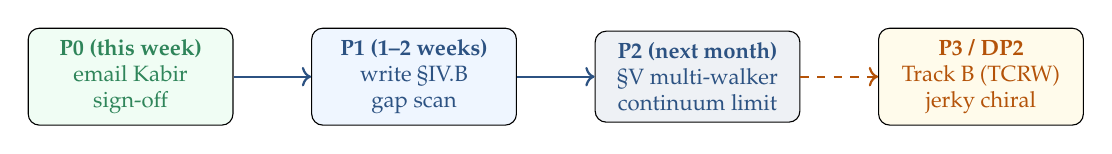
\begin{tikzpicture}[scale=1.0, every node/.style={font=\footnotesize, align=center, inner sep=4pt}]
\node[draw, rounded corners, fill=goodfill, text=good, minimum width=2.6cm] (p0) at (0, 0) {\textbf{P0 (this week)}\\email Kabir\\sign-off};
\node[draw, rounded corners, fill=keyfill, text=accent, minimum width=2.6cm] (p1) at (3.6, 0) {\textbf{P1 (1--2 weeks)}\\write §IV.B\\gap scan};
\node[draw, rounded corners, fill=accent!8, text=accent, minimum width=2.6cm] (p2) at (7.2, 0) {\textbf{P2 (next month)}\\§V multi-walker\\continuum limit};
\node[draw, rounded corners, fill=ideafill, text=idea, minimum width=2.6cm] (p3) at (10.8, 0) {\textbf{P3 / DP2}\\Track B (TCRW)\\jerky chiral};
\draw[->, accent, thick] (p0) -- (p1);
\draw[->, accent, thick] (p1) -- (p2);
\draw[->, idea, thick, dashed] (p2) -- (p3);
\end{tikzpicture}
\end{center}

\subsection*{P0 (this week)}
\begin{itemize}[leftmargin=*,nosep]
\item Email Kabir with the two-bug summary + main figure attached.
\item Get his sign-off on the fix; ask whether the figure /
  derivation goes into the Confinement draft directly or as a
  supplementary note.
\end{itemize}

\subsection*{P1 (next 1--2 weeks)}
\begin{itemize}[leftmargin=*,nosep]
\item Write §IV.B of the Confinement draft properly (one page, plus
  Fig.~11 and a corrected Eq.~B11).
\item Decide on lattice convention for the paper (algebraic $a=b=1$
  vs.\ isotropic $b = \sqrt{3} a$); commit.
\item Compute the gap-closure scan: minimum spectral gap of $M(\vk)$ as
  a function of $\epsilon$ at fixed $\gamma$. Is there a critical
  $\epsilon^*$?
\end{itemize}

\subsection*{P2 (next month)}
\begin{itemize}[leftmargin=*,nosep]
\item §V multi-walker clustering on triangular. Step initial condition,
  look for non-monotonic clustering signature.
\item Continuum limit of $M(\vk)$ for small $\vk$. Derive an effective
  Fokker-Planck-like operator.
\end{itemize}

\subsection*{P3 / DP2 directions}
\begin{itemize}[leftmargin=*,nosep]
\item Track B: TCRW (rotation chirality) on triangular. Build the
  Bloch matrix, scan for gap closure at $\omega = 1/2$ analogue, and
  compute the 2D Zak phase. Open research question.
\item Berry curvature / Chern number on triangular for either Track A
  or Track B once the spectrum is mapped.
\item Connection to jerky chiral active particles (S.~Jose / H.~Löwen
  direction) -- adding third-derivative noise to the same framework.
\end{itemize}

% ===============================================================
\section{Files inventory}\label{sec:inventory}

\begin{center}\small
\renewcommand{\arraystretch}{1.18}
\begin{tabular}{lp{8.5cm}}
\toprule
file & purpose \\
\midrule
{\sf kmc\_triangular\_jmvr.f90} & 100M-walker Fortran KMC, the high-precision ground truth \\
{\sf mt.f90} & Mersenne Twister RNG for Fortran \\
{\sf run\_kmc.sh} & build + run script for the Fortran KMC \\
{\sf kmc\_triangular\_counts.txt} & output histogram, $n_1, n_2,$ count \\
{\sf triangular\_jmvr\_corrected.py} & Python theory: buggy and corrected $M(\vk)$, theory $P$ \\
{\sf forensic\_two\_bugs.py} & 4-way comparison vs Fortran KMC -- the receipt for the two-bug claim \\
{\sf forensic\_pbc\_is\_fine.py} & (historical) original (wrong) test that gave the false ``PBC is fine'' answer \\
{\sf robustness\_check.py} & 3-point parameter robustness test \\
{\sf diagnose\_hexring.py} & 6-fold angular modulation sanity check \\
{\sf fig11\_final\_hex.py} & Fig.~11 replacement script (main + evidence figures) \\
{\sf fig11\_final\_hex.png} & main paper-ready figure \\
{\sf fig11\_final\_hex\_evidence.png} & with residual z-score panel \\
{\sf robustness\_check.png} & 3-point parameter scan figure \\
{\sf jmvr\_single\_walker.html} & interactive JMVR walker (square + triangular) \\
{\sf tcrw\_single\_walker.html} & interactive TCRW walker (square + triangular) \\
{\sf derivation/jmvr\_triangular\_full\_derivation.pdf} & 18-page formal derivation \\
{\sf derivation/jmvr\_triangular\_project\_report.pdf} & this document \\
\bottomrule
\end{tabular}
\end{center}

% ===============================================================
\section{Acknowledgements}\label{sec:thanks}

\begin{itemize}[leftmargin=*,nosep]
\item \textbf{Kabir Ramola} (PI, TIFR Hyderabad) -- for the problem,
  the geometric intuition about the skew PBC, and pointing at the
  unfinished draft as a real project rather than a textbook exercise.
\item \textbf{Mustansir Barma} (TIFR Hyderabad) -- co-author of the
  2021 draft and the 2022 JMVR paper; the foundational model is his
  group's.
\item \textbf{Dipanjan Mandal} (formerly TIFR Hyderabad) -- whose 2019
  Mathematica notebook gave us the structure to work from, including
  the two bugs we fixed.
\item \textbf{Stephy Jose} (Heinrich-Heine-Universität Düsseldorf,
  with H.~Löwen) -- co-author of the 2022 JMVR paper; potential
  collaborator on the jerky chiral direction for DP2.
\end{itemize}

% ===============================================================
\section{Closing}\label{sec:closing}

This work converts a five-year-old abandoned project into a sharply
diagnosed, fully verified result. The two bugs in
{\sf{rtp\_tl\_2.nb}} and the Confinement-2021 draft are now isolated
and fixed. The corrected theory matches a 100M-walker Fortran KMC at the
Monte Carlo noise floor.

The next moves -- write up §IV.B, scan for gap closure, attempt §V
multi-walker, open Track B -- are well-defined and tractable. The
infrastructure (Fortran KMC, Python theory, diagnostic scripts,
visualisations) is in place and can be reused for all of them.

\vspace{1cm}
\noindent\hrulefill\\[2mm]
\footnotesize\noindent
\textit{Companion document:} \emph{The JMVR active random walker on the
triangular lattice -- a complete derivation, two bugs, and a
verification protocol} (18 pages, same folder).

\end{document}
